\documentclass[10pt]{beamer}
\usepackage[french]{babel}

\mode<presentation> {
\usetheme{AnnArbor}
\usecolortheme{beaver}
}

\usepackage{graphicx} % Allows including images
\usepackage{booktabs} % Allows the use of \toprule, \midrule and \bottomrule in tables
\usepackage[utf8]{inputenc}
\usepackage{bm}

%----------------------------------------------------------------------------------------
%	TITLE PAGE
%----------------------------------------------------------------------------------------

\title[Effet bilame]{Effet bilame (bimetallic strip)}
\author[Groupe 4]{Fakri Yassir, Karroucha Wissam, Mazé François, Pollet Florent} % Your name
\institute[Mines Paris] % Your institution as it will appear on the bottom of every slide, may be shorthand to save space
{
Mines ParisTech \\ % Your institution for the title page
}
\date{\today} % Date, can be changed to a custom date

\begin{document}

\begin{frame}
\titlepage % Print the title page as the first slide
\begin{figure}
    \centering
    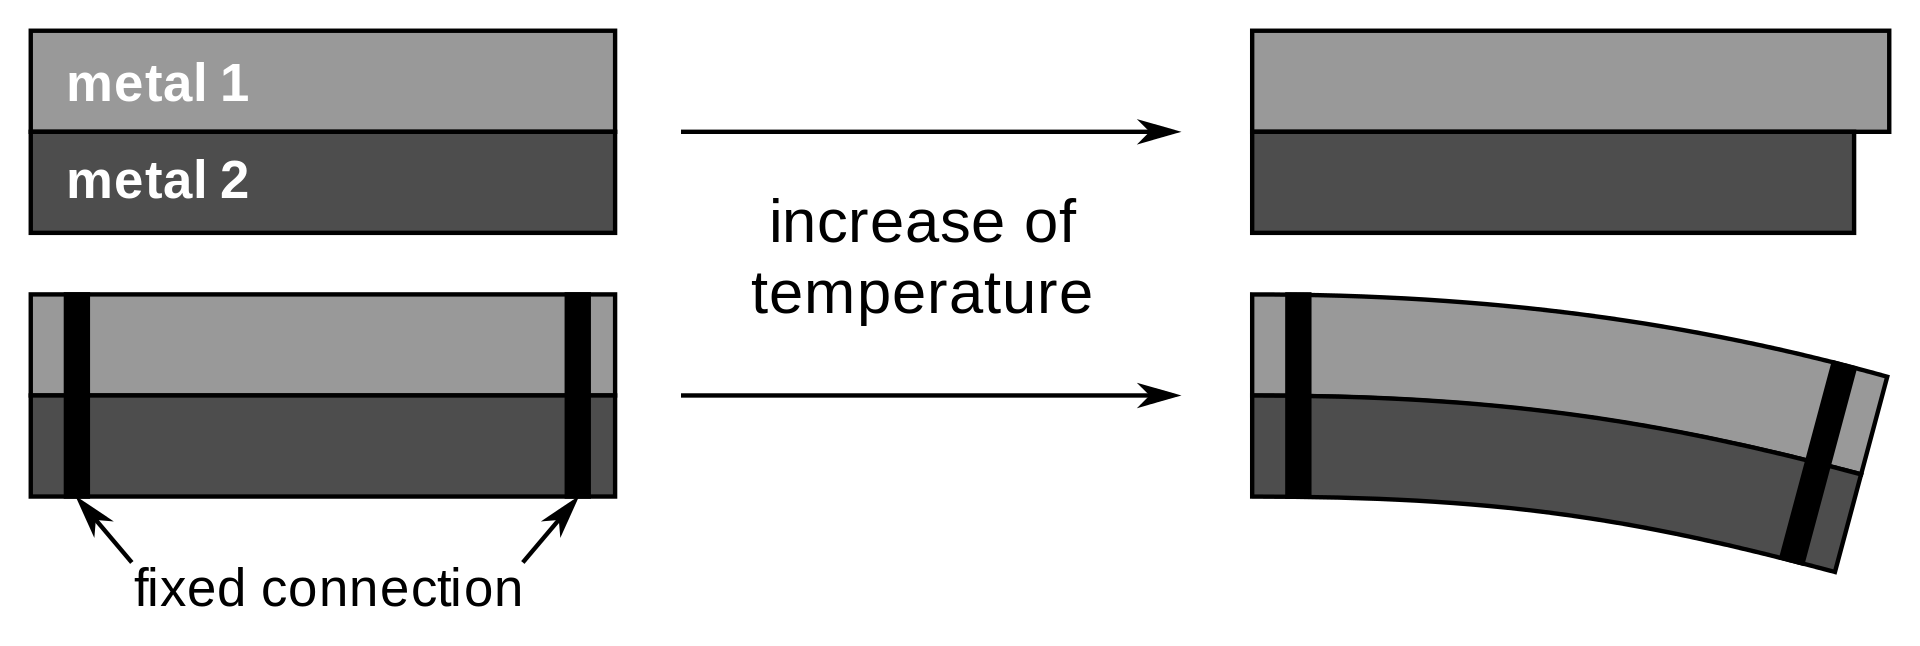
\includegraphics[scale=0.1]{imgs/bilame.png}
\end{figure}
\end{frame}

\begin{frame}
\frametitle{Plan} % Table of contents slide, comment this block out to remove it
\tableofcontents % Throughout your presentation, if you choose to use \section{} and \subsection{} commands, these will automatically be printed on this slide as an overview of your presentation
\end{frame}

%----------------------------------------------------------------------------------------
%	PRESENTATION SLIDES
%----------------------------------------------------------------------------------------
\section{Effet bilame} % Sections can be created in order to organize your presentation into discrete blocks, all sections and subsections are automatically printed in the table of contents as an overview of the talk
%------------------------------------------------

\subsection{Contraintes équi-biaxiales} 
\subsection{Déformations des couches} 
\subsection{Equations de compatibilité} 
\subsection{Déplacements} 
\subsection{Contraintes dans chaque couche} 

\input{part_2_françois.tex}


%------------------------------------------------
\section{Mécanique des microsystèmes} % Sections can be created in order to organize your presentation into discrete blocks, all sections and subsections are automatically printed in the table of contents as an overview of the talk
%------------------------------------------------


\subsection{La formule de Stoney} % A subsection can be created just before a set of slides with a common theme to further break down your presentation into chunks

\begin{frame}
    \frametitle{Contexte et rappels}
    \begin{itemize}
        \item En ce qui concerne la mécanique des microsystèmes...
        \item Deux matériaux quelconques
        \item Petites déformations (HPP)
        \item $\bm{u} = (AX_1X_3 + CX_1)\bm{e_1} + (AX_2X_3 + CX_2)\bm{e_2} + (-\frac{A}{2}\left[X_1^2+X_2^2\right]-\frac{2\nu}{1-\nu}\left[\frac{A}{2}X_3^2+CX_3\right]+\frac{1+\nu}{1-\nu}\alpha\left[T-T_0\right]X_3)\bm{e_3}$
        \item $A = 6\frac{M_fh_f}{M_sh_s^2}(\alpha_f-\alpha_s)(T-T_0)(1+\frac{h_f}{h_s})\Delta^{-1}$
        \item $\Delta = 1+4\frac{M_fh_f}{M_sh_s}+6\frac{M_fh_f^2}{M_sh_s^2}+4\frac{M_fh_f^3}{M_sh_s^3}+\frac{M_f^2h_f^4}{M_s^2h_s^4}$
        \item $C = \Delta^{-1}(T-T_0)\left[\alpha_s + 4 \alpha_f \frac{M_fh_f}{M_sh_s} + 3 (\alpha_s + \alpha_f)\frac{M_fh_f^2}{M_sh_s^2} + 4\alpha_s \frac{M_fh_f^3}{M_sh_s^3} + \alpha_f \frac{M_f^2h_f^4}{M_s^2h_s^4}  \right]$
    \end{itemize}
\end{frame}

% 30s
    
\begin{frame}
    \frametitle{La formule de Stoney (1909)}
    
    \begin{figure}
        \centering
        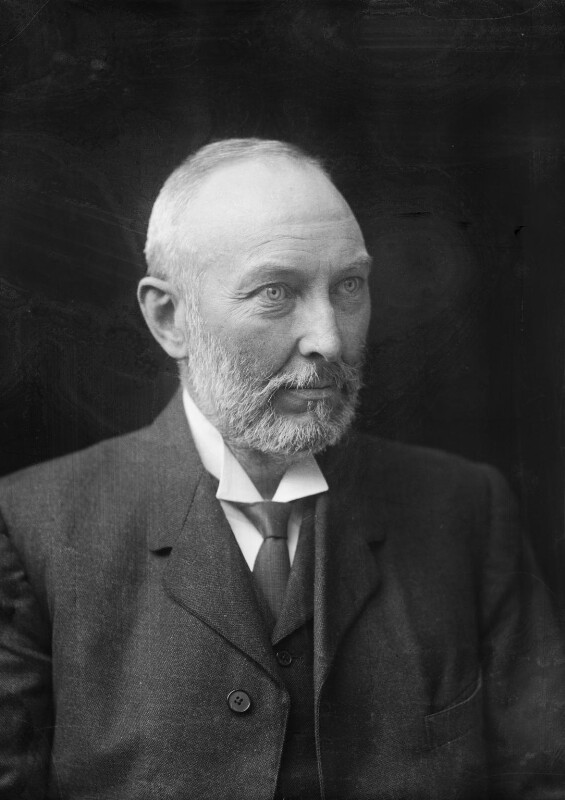
\includegraphics[scale=0.07]{imgs/stoney.jpg}
        \caption{George Gerald Stoney (1863-1942)}
    \end{figure}

    \begin{itemize}
        \item Supposons que $\frac{h_f}{h_s} \ll 1$
        \item Quelle est la courbure $c$ prise par l'ensemble ?
    \end{itemize}
    
    \begin{figure}
        \centering
        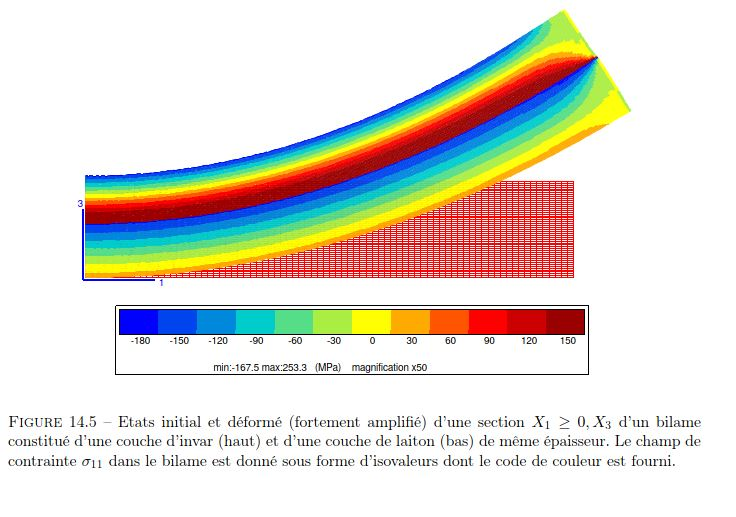
\includegraphics[scale=0.2]{imgs/deformation.JPG}
        \caption{Résultat de simulation}
    \end{figure}
    
\end{frame}


% 1m

\begin{frame}
    \frametitle{La formule de Stoney (1909)}

    \begin{itemize}
        \item $c = 6\frac{M_fh_f}{M_sh_s^2}(\alpha_s-\alpha_f)(T-T_0)$ si $M_fh_f \ll M_sh_s$ 
        \item Dans les autres directions ? Courbure nulle ou parabolique
        \item Permet de prévoir la déformation de l'ensemble, en combinant ls caractéristiques géométriques et les propriétés mécaniques des couches
    \end{itemize}
    
    \begin{figure}
        \centering
        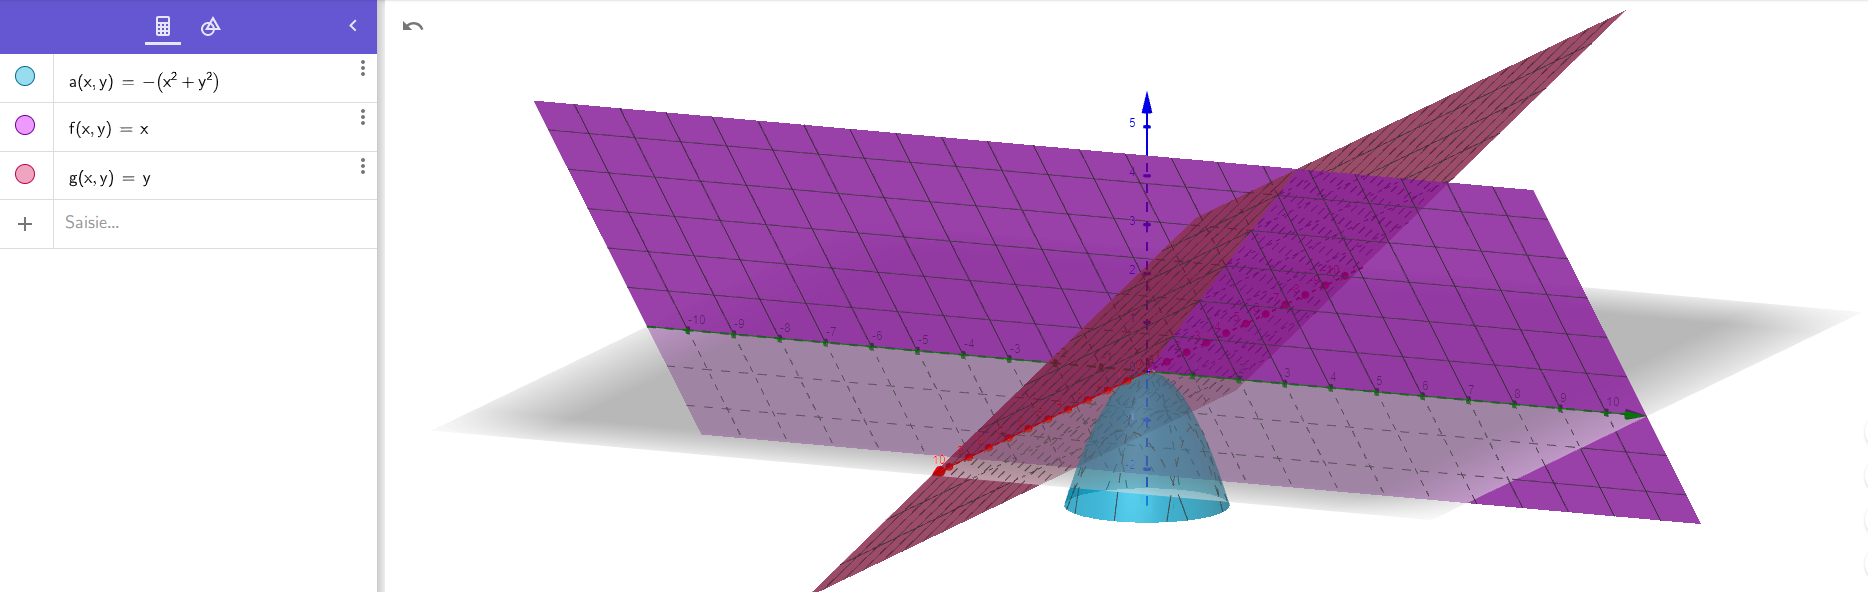
\includegraphics[scale=0.25]{imgs/courbes.png}
        \caption{Paraboloïde de révolution et hyperplans}
    \end{figure}
    
\end{frame}

% 4m15

\begin{frame}
    \frametitle{La formule de Stoney (1909)}

    \begin{itemize}
        \item Qu'évoquait l'article de Stoney ?
        \item Une formule estimant sous certaines conditions (précédemment évoquées) pour déterminer en mesurant la tension et la courbure la couche de nickel déposée sur une électrode 
        \item Reliait la valeur des contraintes à la courbure de l'électrode avec son dépôt
        \item Formule 2D améliorée par Berry en 1988
    \end{itemize}
    
\end{frame}

% 4m45

\begin{frame}
\frametitle{Expérience sommaire : présentation}
\begin{itemize}
    \item Découper des bandes (8 cm par 1 cm environ)
    \item Feuille d'aluminium : $\alpha_f = 23 \times 10^{-6} K^{-1}$, $h_f = 0.02 mm$, $E_f = 62 GPa$, $\nu_f = 0.35$
    \item Papier bristol : $\alpha_s = 3 \times 10^{-6} K^{-1}$, $h_s = 0.3 mm$, $E_s = 3 GPa$, $\nu_s = 0.2$
    \item Colle pour fixer les deux morceaux
    \item Bougie : $T = 200$ °C (juste en-dessous de la température d'auto-inflammation du papier) et $T_0 = 25$ °C
    \item C'est parti !
\end{itemize}
\end{frame}

% 6m

\begin{frame}
\frametitle{Expérience sommaire : résultats}
    \begin{itemize}
        \item Les se dilatent différemment sous l'effet de la chaleur
        \item On remarque que c'est l'aluminium qui est sur la face externe de la courbure. 
        \item On est bien dans le cas des petites déformations avec $||Grad(\underline{u})|| \ll 1$.
        \item On peut chercher à vérifier le signe de la courbure dans la formule de Stoney, même si la deuxième hypothèse $M_f h_f << M_s h_s$ n'est pas vraiment vérifiée :
        \begin{itemize}    
            \item $T-T_0 > 0$
            \item $\alpha_s - \alpha_f < 0$
            \item Donc $c < 0$ (la courbure est vers le bas)
        \end{itemize}
        \item Diversité des applications de cet effet (ici, Stoney, électronique)
    \end{itemize}
\end{frame}

%6m30


\subsection{Contraintes dans un film mince sur un substrat} % A subsection can be created just before a set of slides with a common theme to further break down your presentation into chunks

\begin{frame}
\frametitle{Forme simplifiée des contraintes sous les hypothèses de Stoney}
\begin{itemize}
    \item Contrainte moyenne : $\bar{\sigma}_{11}=\frac{1}{h}\int\sigma_{11}\rm{d}X_3$
    \item Développons au premier ordre $\Delta$, $C$ et $A$
    \item $\sigma_{11}^f=M_f(AX_3+C-\alpha_f(T-T_0)) \approx M_f (\alpha_s - \alpha_f)(T-T_0)$
    \item $\sigma_{11}^s=M_s(AX_3+C-\alpha_s(T-T_0)) \approx \frac{M_fh_f}{M_sh_s} (\alpha_f-\alpha_s)(T-T_0)(6\frac{X_3}{h_s}+4)$
\end{itemize}
\end{frame}

% 8m

\begin{frame}
    \frametitle{Forme simplifiée des contraintes sous les hypothèses de Stoney}
    \begin{itemize}
        \item Par équi-biaxialité, $\bar{\sigma}_{11}^f=\bar{\sigma}_{22}^f=M_f(\alpha_s-\alpha_f)(T-T_0)$, ce qui est un résultat remarquable (ne dépend pas de la géométrie ni des propriétés élastiques du substrat, que de propriétés thermoélastiques du film et du désaccord de dilatation)
        \item De même, $\bar{\sigma}_{11}^s=\bar{\sigma}_{22}^s=M_f\frac{h_f}{h_s}(\alpha_f-\alpha_s)(T-T_0)$
        \item La contrainte moyenne est donc nulle (cohérent car il n'y a pas de chargement extérieur et l'on est en statique, que des contraintes locales à l'intérieur)
        \item Quelle est la fibre neutre ?
    \end{itemize}
\end{frame}

% 9m15

\begin{frame}
    \frametitle{Fibre neutre}
    \begin{itemize}
        \item $\sigma_{11}^s=0 \implies X_3 \simeq \frac{-2h_s}{3}$ (cohérent, bien dans le substrat, car contrainte constante dans le film)
        \item Confirmation par représentation graphique et l'article de Stoney (pas le cas pour l'exemple de la partie précédente)
    \end{itemize}
\end{frame}

% 10m

\subsection{Application des conditions de Stoney}

\begin{frame}
    \frametitle{Dépôt d'aluminium sur un substrat de silicium}
    On étudie ici
les contraintes qui se développent dans un film d’aluminium d’1 µm d’épaisseur déposé sur un substrat
de silicium de 500 µm d’épaisseur.
    \begin{itemize}
        \item Le dépôt s’effectue à une température de 50$^{\circ}C$
        \item A la fin du dépôt, le substrat et le film sont supposés être dans leur état naturel.
        \item le composant est un disque parfait de rayon égal à 200mm.
        \item Il est ensuite refroidi jusqu’à la température ambiante de 20$^{\circ}C$.
    \end{itemize}
\end{frame}

\begin{frame}
    \frametitle{Calcul de la courbure et des contraintes}
    Les hypothèses de Stoney sont remplies:
    $$\frac{h_{f}}{h_{s}} = 2.10^{-3},   ~ ~ ~ \frac{M_{f}h_{f}}{M_{s}h_{s}} = 1,1.10^{-3}$$
    On peut donc appliquer la formule de Stoney pour déterminer la courbure du bilame :
    $$c = 8,3.10^{-3} m^{-1} ~ et ~ R = \frac{1}{c}=120m$$
    \begin{figure}
        \centering
        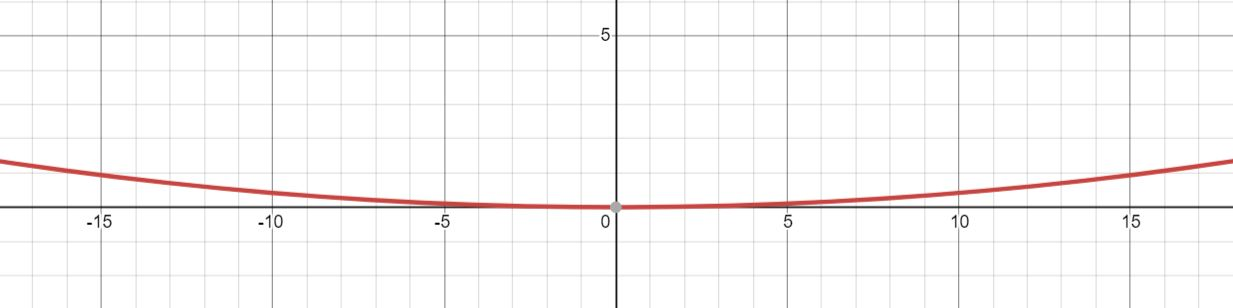
\includegraphics[scale=0.4]{imgs/courbure positive.JPG}
    \end{figure}
\end{frame}

\begin{frame}
    \frametitle{Calcul de la courbure et des contraintes}
    L'expression de la courbure permet d'accéder à une estimation de la contrainte moyenne dans le film : 
    $$ \sigma_{11}^{f} = \frac{M_sh_s^2}{6h_f}\cdot c $$
    Donc:
    $$ \sigma_{11}^{f} = 63 MPa ~~~ et ~~~ \sigma_{11}^{s} = -0.13 MPa $$ 
\end{frame}

\begin{frame}
    \frametitle{Méthodes de mesure de la courbure}
    \textbf{\Large{Méthode mécanique (Profilomètre)}}
    \begin{itemize}
        \item Le but c'est d'enregistrer le déplacement $u_3$ et d'en déduire la courbure
    \end{itemize}
    \begin{figure}
        \centering
        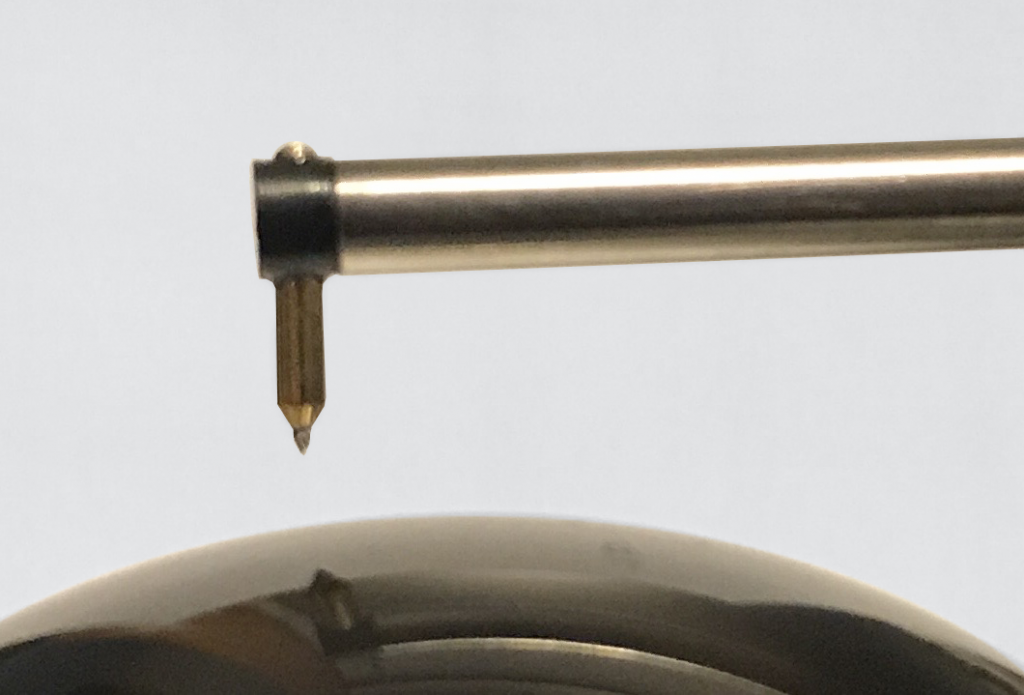
\includegraphics[scale=0.2]{imgs/Digital_Metrology-Measuring_Arcs_with_Stylus_1_Stylus_on_Ball-1024x695.png}
    \end{figure}
\end{frame}

\begin{frame}
    \frametitle{Méthodes de mesure de la courbure}
    \textbf{\Large{Méthode de diffraction X-Ray}}
    \begin{figure}
        \centering
        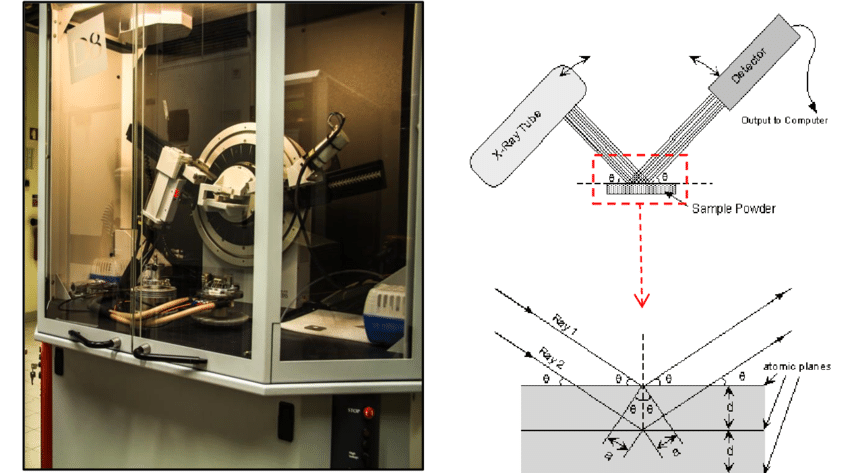
\includegraphics[scale=0.3]{imgs/XRD-equipment-and-schematic-of-X-ray-diffraction-adopted-from-Erdem-2012-Nelson-2015.png}
    \end{figure}
\end{frame}

\begin{frame}
    \frametitle{Méthodes de mesure de la courbure}
    \begin{itemize}
        \item Cette méthode détermine successivement l'angle de Bragg pour l'intensité de diffraction maximale à différents emplacements radiaux de la surface du substrat.
        \item Le rayon de courbure du substrat est la distance radiale entre les deux endroits de la surface où sont effectuées les mesures de diffraction, divisée par la différence des positions angulaires des maxima d'intensités.
    \end{itemize}
    $$R = \frac{1}{c} = \frac{r_2-r_1}{\theta _2-\theta_1}$$
\end{frame}

\begin{frame}
    \frametitle{Méthodes de mesure de la courbure}
    \textbf{\Large{Méthode optique}}
    \begin{itemize}
        \item Un faisceau laser incident sur la surface du substrat est balayé le long d'une ligne droite.
        \item La déviation angulaire 2$\theta$ du faisceau réfléchi par rapport à l'incident est mesurée en fonction de la distance $r$ par rapport à un point de référence.
        \item La déviation du faisceau balayé est surveillée par un détecteur sensible à la position.
        \item La courbure est liée à l'angle $\theta$ qui dépend de $r$.
    \end{itemize}
    \begin{figure}
        \centering
        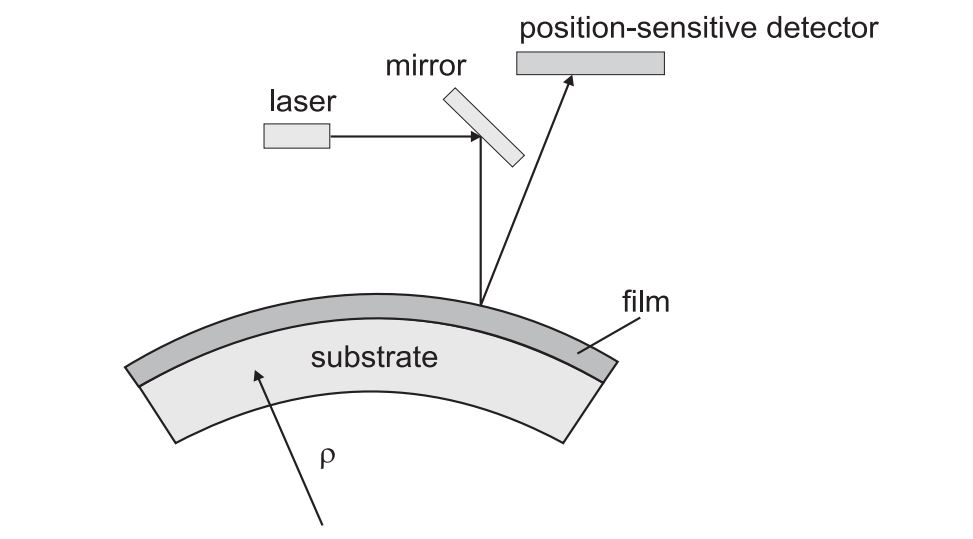
\includegraphics[scale=0.3]{imgs/laser method.JPG}
    \end{figure}
\end{frame}

\begin{frame}
    \frametitle{Contraintes d'épitaxie}
    \textbf{\Large{C'est quoi l'épitaxie ?}}
    \begin{itemize}
        \item C'est une technique de croissance orientée, de 2 cristaux possédant un certain nombre d'éléments de symétrie communs dans leurs réseaux cristallins.
        \item Elle est utilisée pour faire croître des couches minces, de quelques nanomètres d'épaisseur. Pour cela, des atomes sont déposés sur la surface parfaitement polie d'un monocristal, le substrat.
        \item Le substat est choisi de façon à avoir des paramètres de maille proches de ceux du cristal qui souhaite être obtenu.
    \end{itemize}
    Il y a deux types d'épitaxie:
    \begin{itemize}
        \item homoépitaxie   : les 2 matériaux sont identiques.
        \item hétéroépitaxie : les 2 matériaux sont différents.
    \end{itemize}
    Dans le 2ème type, la croissance n'est possible que s'il y a accord de maille, c'est-à-dire qu'il aient le même réseau cristallin et que les paramètres de maille soient assez voisins.
    
\end{frame}

\begin{frame}{Contraintes d'épitaxie}
    \begin{itemize}
        \item La différence des paramètres de maille induit une contrainte dans le plan de base.
        \item Le film se déforme pour avoir le même paramètre de maille que le substrat, donc il n'y a pas de déformation ni de contrainte dans le substrat.$$ \varepsilon _{11} ^{\star s} = 0 $$
        \item Toutefois, ceci n'est pas réaliste puisque aucune contrainte dans le substrat n'équilibre la contrainte dans le film. $\Rightarrow$ Il faut introduire un modèle élastique multicouche pour décrire les déformations présentes lors de la croissance du film sur le substrat.
    \end{itemize}
\end{frame}

\begin{frame}{Contraintes d'épitaxie}
    \begin{itemize}
        \item Ici on prend le cas par exemple des dépôts de silicium–germanium sur un substrat de silicium monocristallin.
        \item le paramètre cristallin $a_{SiGe} = 0.5476$nm du silicium–germanium (pour 80$\%$ de silicium et 20$\%$ de germanium dans le composé binaire) est légèrement plus grand que le paramètre du silicium $a_{Si} = 0.5431$nm en raison de l’implantation des atomes de germanium.
        \item Si le film n’était pas contraint de croître en épitaxie avec le substrat, il se déformerait librement de la quantité:
        $$\varepsilon _{11} ^{\star f} = \varepsilon _{22} ^{\star f} = \varepsilon _{33} ^{\star f} = \frac{a_{SiGe}-a_{Si}}{a_{Si}}  $$
        \item La déformation totale dans le film est donc la somme d’une déformation élastique et de la déformation libre d’épitaxie :
        $$\varepsilon _{11} ^{f} = \varepsilon _{11} ^{ef} + \varepsilon _{11} ^{\star f}$$
    \end{itemize}
\end{frame}

\begin{frame}{Contraintes d'épitaxie}
    \begin{itemize}
        \item Données : $M_f$ = 170 GPa , $h_f$ = 100 nm , $h_s$ = 1 mm
        \item La déformation libre d’épitaxie s’apparente à la dilatation thermique et l’on a l’analogie suivante :
        $$\frac{a_{SiGe}-a_{Si}}{a_{Si}} \equiv \alpha _f(T-T_0) ~~ et ~~ 0 \equiv \alpha _s(T-T_0)$$
        Donc: $$\frac{a_{SiGe}-a_{Si}}{a_{Si}} = 0.83\%$$
        \item $$\bar{\sigma}_{11}^{f} = \bar{\sigma}_{22}^{f} \simeq M_f \frac{a_{SiGe}-a_{Si}}{a_{Si}} = -1403MPa$$
        $$c = \frac{6M_fh_f}{M_sh_s^2}\cdot \frac{a_{SiGe}-a_{Si}}{a_{Si}} = -5,6\cdot 10^{-3}m^{-1}$$
        Ce qui donne le rayon de courbure : $R=-177m$
        \item Nous remarquons qu'ils y a des contraintes de compression conséquentes qui règnent sur le film après élaboration.
    \end{itemize}
\end{frame}

\begin{frame}{Expérience}
    \begin{itemize}
        \item On a réalisé un bilame en superposant un morceau de ruban adhésif sur un bout de papier. Lorsqu'on le plonge dans l'eau froide, on voit le bilame s'enrouler, le côté papier à l'extérieur.
    \end{itemize}
    \begin{figure}
        \centering
        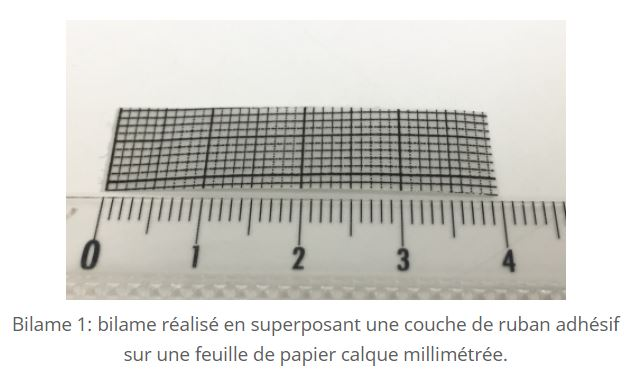
\includegraphics[scale=0.3]{imgs/exp1.JPG}
    \end{figure}
    \begin{figure}
        \centering
        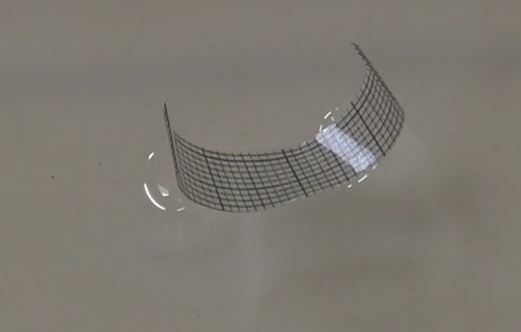
\includegraphics[scale=0.3]{imgs/exp2.JPG}
    \end{figure}
\end{frame}

\begin{frame}{Expérience}
    \begin{figure}
        \centering
        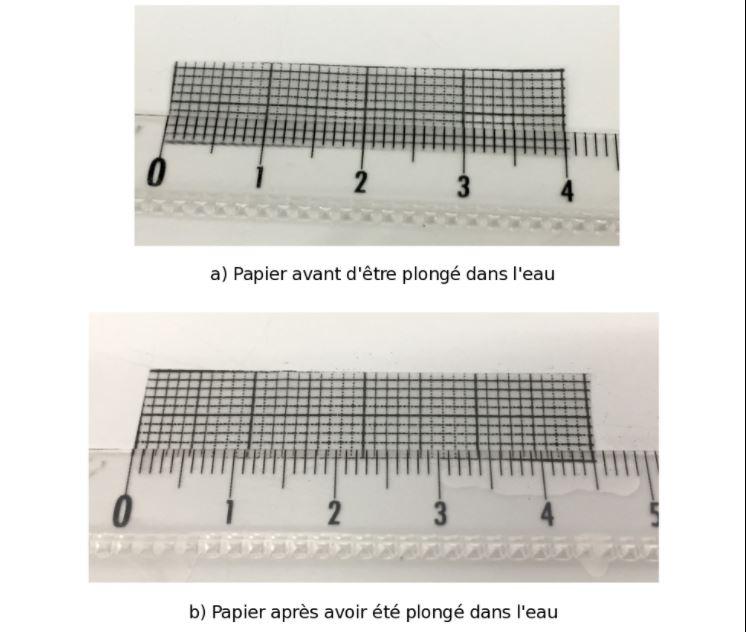
\includegraphics[scale=0.3]{imgs/exp3.JPG}
    \end{figure}
    \begin{itemize}
        \item On constate que le papier s'est dilaté dans l'eau. Par contre, la taille du ruban adhésif reste la même. La dilatation d'un des côtés du bilame provoque une déformation de celui-ci.
    \end{itemize}
    
\end{frame}


\begin{frame}
    \Huge{\centerline{Merci ! Des questions ?}}
\end{frame}
    
\end{document} 